\section{Gazpacho}
\begin{tikzpicture}[remember picture,overlay]
    \node[anchor=east,yshift=-4.5cm,inner sep=0pt] at (current page text area.east|-0,3cm) {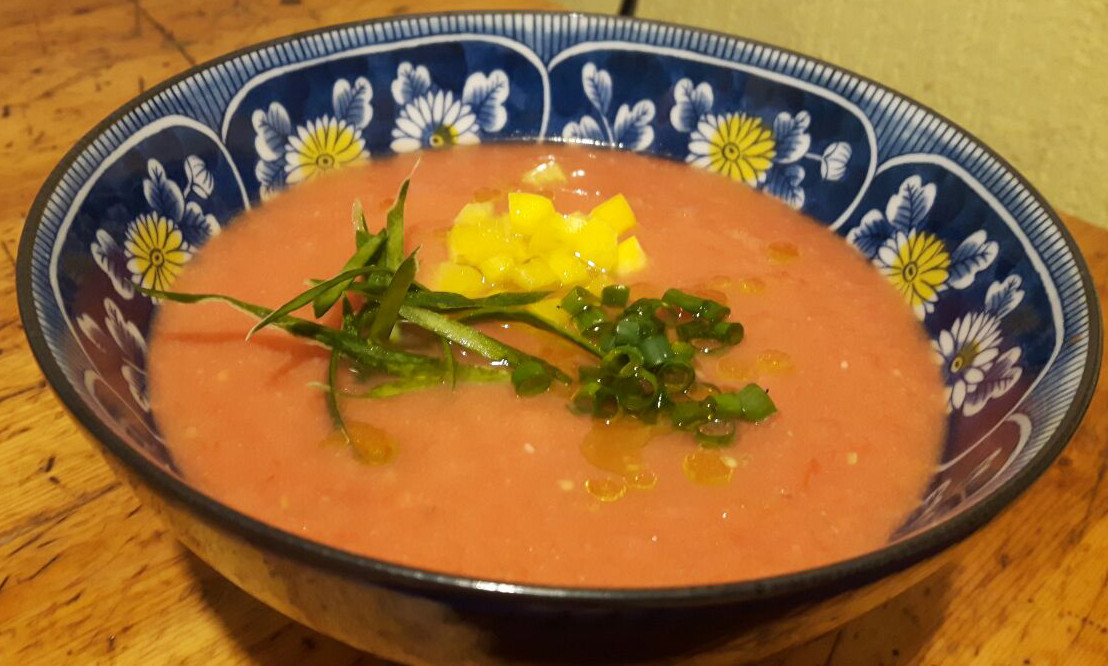
\includegraphics[height=4.5cm]{res/Gazpacho.jpg}};
\end{tikzpicture}
\begin{longtable}{rlL{16.46cm}}
    1       &   Gurke               &   schälen, entkernen und schneiden.
                                        Von\\
    1kg     &   Tomaten             &   die Stiele entfernen und schneiden.\\
    1       &   Paprika             &   entkernen, schneiden und einen Teil zum dekorieren\\
            &                       &   zur Seite legen.\\
    50g     &   Weißbrot            &   zerkleinern und alles zusammen mit\\
    2 EL    &   Essig               &   (Sherry oder Weißwein),\\
    3 EL    &   Olivenöl            &   und\\
    1 TL    &   Salz                &   pürieren.\\
    1 Zehe  &   Knoblauch           &   klein schneiden und dazugeben.\\
    2       &   Frühlingszwiebeln   &   schneiden und den weißen Teil dazugeben.
                                        Noch einmal kurz pürieren.\\
\end{longtable}
Das Weißbrot kann für eine dünnere Konsistenz weggelassen werden.
Ggf. kann man hierfür auch noch Eiswasser mitpürieren.
Man kann das Gazpacho auch mit Cumin verfeinern oder den Knoblauch weglassen, wenn man ein anderes Aroma möchte.
Gazpacho wird kalt serviert.